\section{Development Workflow}
The development workflow for this thesis combines a local machine for code authoring, a cloud GPU instance for training, and cloud storage for data and artefact persistence. This hybrid design is necessitated by the absence of local GPU compute: the primary development machine was an Apple M1 MacBook Air through May 2026 and a Windows PC with PyCharm from June 2026, while the EAV modality encoders require a GPU for training within a practical time budget.

The workflow's three components---the local CPU machine for code authoring, Google Colab Pro on an NVIDIA L4 GPU for training and inference, and Google Drive for persistent storage of pickles, checkpoints, logits, and results---are illustrated in Figure~\ref{fig:workflow}. The GitHub repository mediates between the local machine and the Colab session, providing version control and a controlled mechanism for code to reach the cloud environment.

\begin{figure}[htbp]
\centering
\IfFileExists{images/fig_5_1_workflow.png}{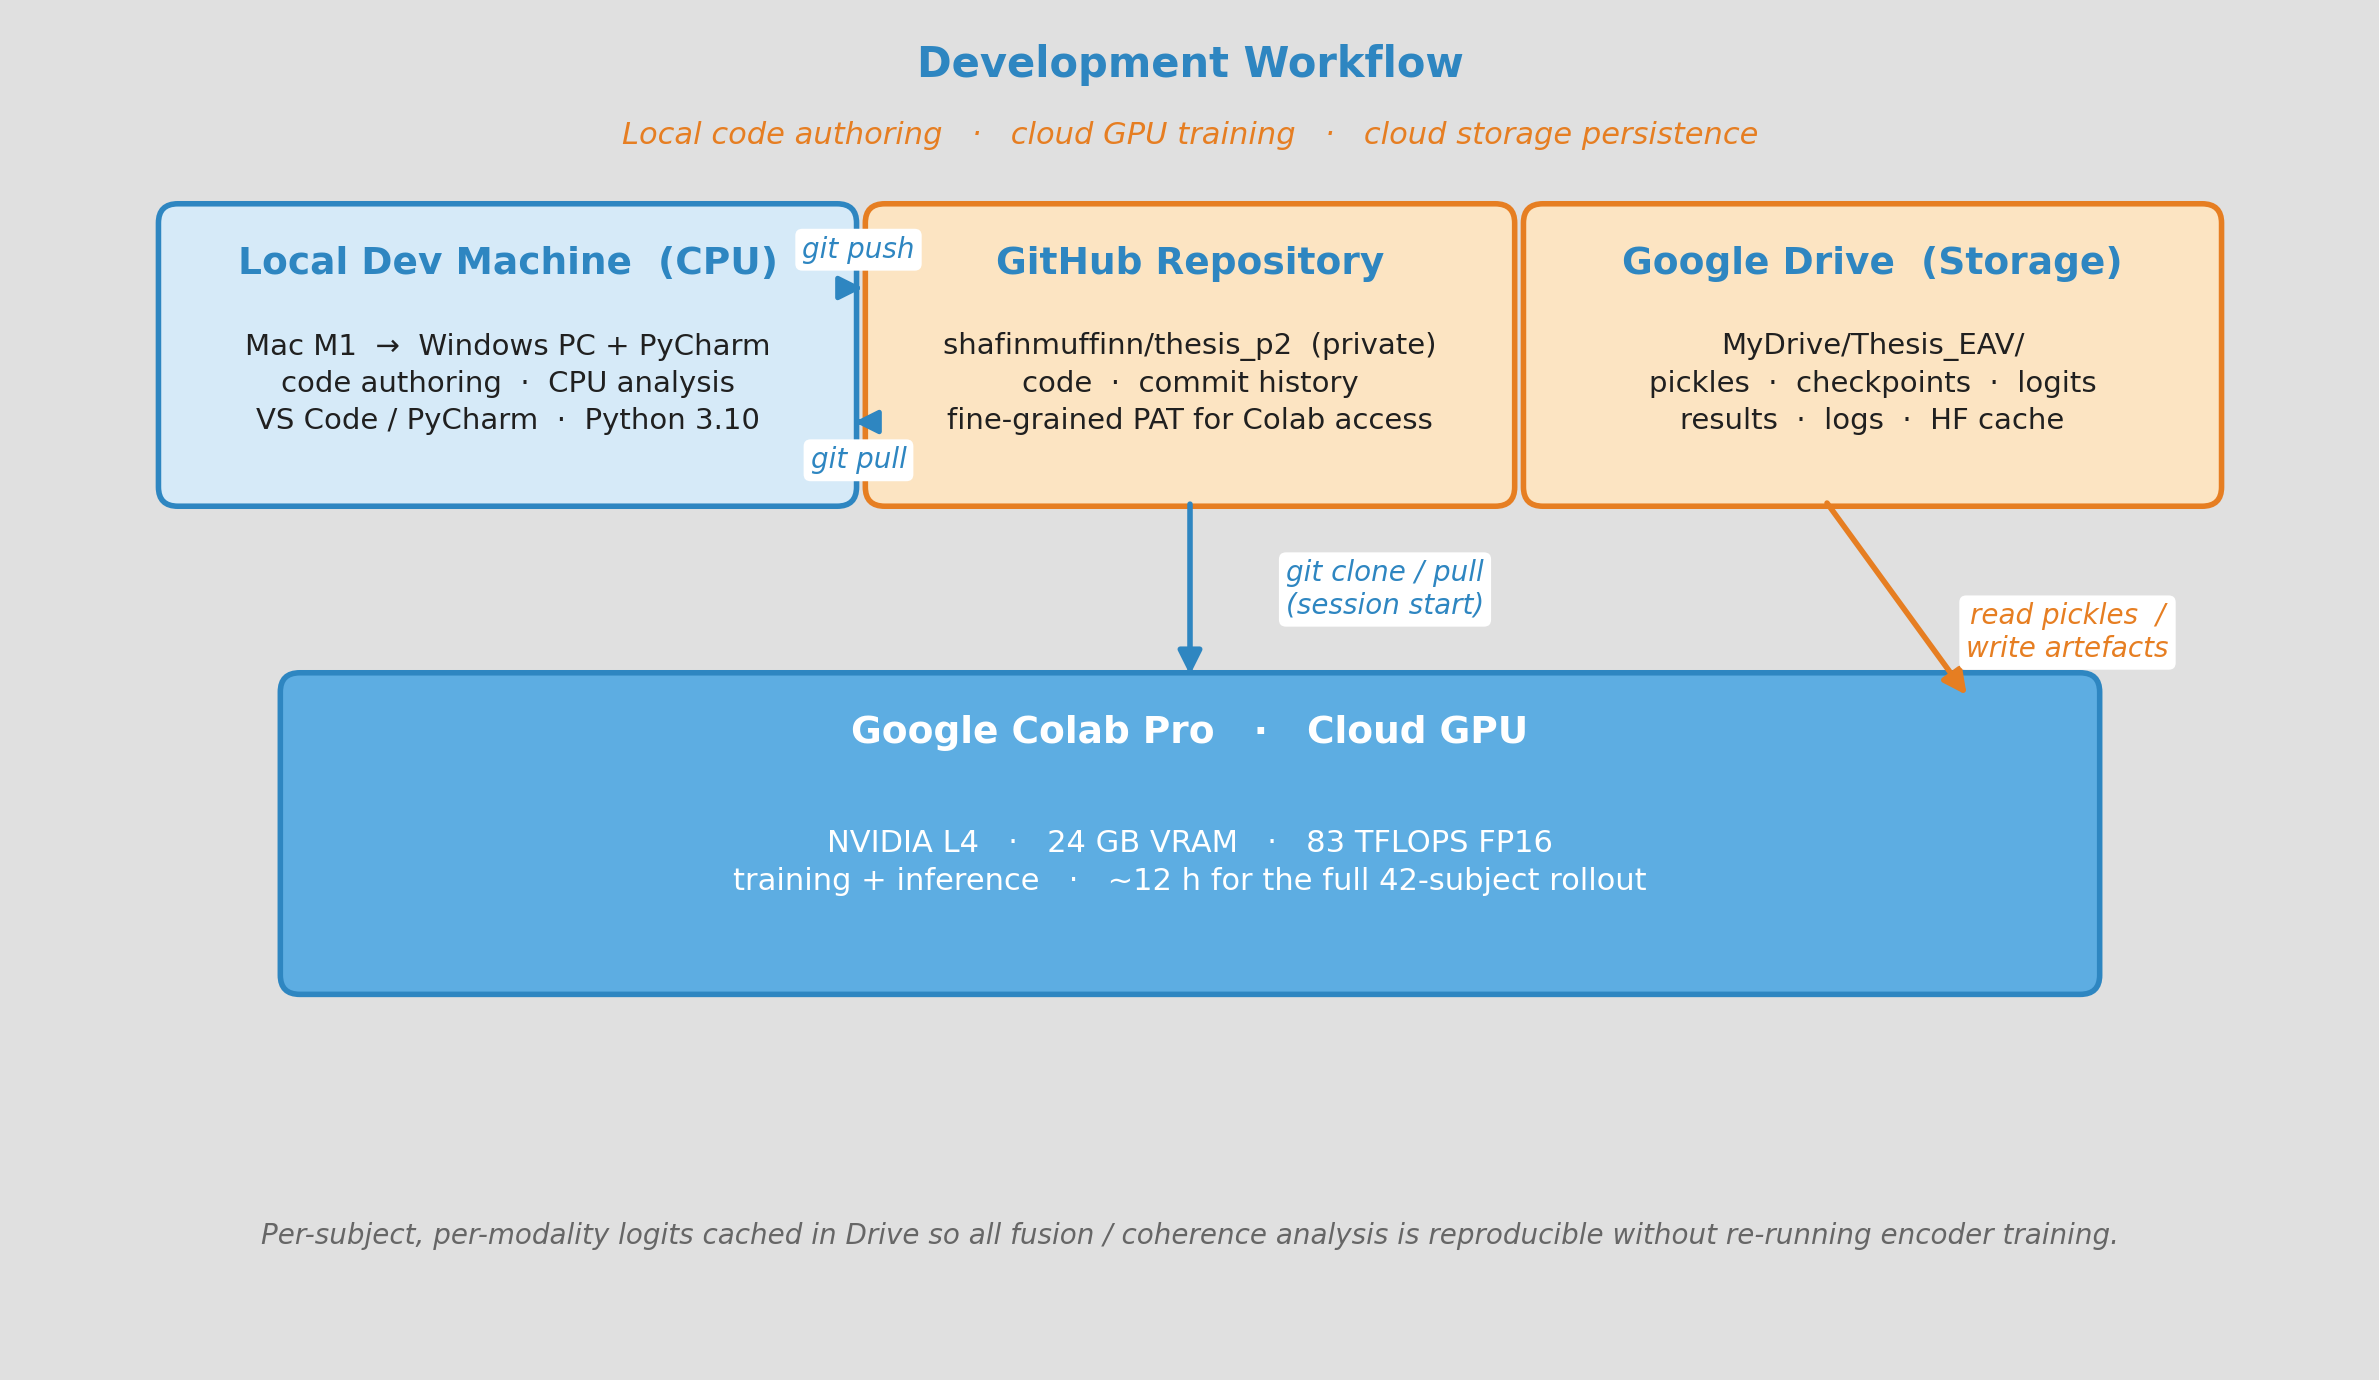
\includegraphics[width=\textwidth]{images/fig_5_1_workflow.png}}{\fbox{\parbox{0.86\textwidth}{\centering Missing image placeholder: \texttt{images/fig\_5\_1\_workflow.png}. Place the three-component workflow diagram here.}}}
\caption{Three-component development workflow. The local CPU machine (left) authors code that is committed and pushed to a private GitHub repository (top); each Colab session clones the repository to gain a fresh copy of the code. Google Colab Pro (centre) runs all training and inference on an NVIDIA L4 GPU. Google Drive (right) stores all bulk data and artefacts (pickles, checkpoints, logits, results, logs), with Colab reading pickles and writing artefacts back to Drive throughout the session.}
\label{fig:workflow}
\end{figure}

\textbf{Local development.} Code is authored locally and committed to a private GitHub repository, \texttt{shafinmuffinn/thesis\_p2}. The Mac M1 development environment with Visual Studio Code and Python 3.10 was used from project inception through 5 May 2026. From 6 May 2026, development switched to a Windows PC using PyCharm and Python 3.10 under a collaborator GitHub account. All code runs identically in both environments.

\textbf{Cloud compute.} Google Colab Pro with an NVIDIA L4 GPU, 24 GB VRAM, and 83 TFLOPS FP16 is the primary training environment. Each Colab session begins with a short setup ritual:
\begin{enumerate}
    \item Mount Google Drive.
    \item Clone or pull the GitHub repository using a fine-grained personal access token stored in Drive.
    \item Set environment variables \texttt{THESIS\_ROOT}, \texttt{EAV\_PICKLES}, \texttt{CHECKPOINTS}, \texttt{RESULTS}, \texttt{LOGS}, \texttt{PRETRAINED}, and \texttt{HF\_HOME} to point at the mounted Drive directories.
    \item Install additional Python packages required in Colab: \texttt{transformers} and \texttt{wandb}; NumPy, SciPy, PyTorch, scikit-learn, librosa, and OpenCV are available in the Colab environment.
    \item Verify directory creation and CUDA availability before launching training.
\end{enumerate}

\textbf{Persistent storage.} Google Drive hosts all bulk data, checkpoints, logits, and results. The Drive layout is:

\begin{verbatim}
MyDrive/Thesis_EAV/
|-- Input_images/
|   |-- Audio/subject_{01..42}_aud.pkl
|   |-- Vision/subject_{01..42}_vis.pkl
|   `-- EEG/subject_{01..42}_eeg.pkl
|-- checkpoints/
|   |-- day5_state_dicts/sub{NN}_{modality}.pt
|   |-- day5_features/sub{NN}.npz
|   `-- day5_per_modality_logits/sub{NN}_{modality}.npz
|-- results/
|   |-- day5_fusion.csv
|   |-- day3_late_fusion.csv
|   |-- suppression_matrix.csv
|   `-- suppression_per_subject.csv
`-- pretrained/hf_cache/
\end{verbatim}

This layout ensures that any session termination loses only the in-progress computation for the current subject, not completed subjects' results.

\section{Path Configuration}
\label{sec:path_configuration}
A single module, \texttt{paths.py}, is the source of truth for all filesystem paths in the project. All paths are resolved from environment variables at module import time:

\begin{verbatim}
THESIS_ROOT = Path(os.environ["THESIS_ROOT"])
EAV_PICKLES = Path(os.environ.get("EAV_PICKLES", THESIS_ROOT / "Input_images"))
CHECKPOINTS = Path(os.environ.get("CHECKPOINTS", THESIS_ROOT / "checkpoints"))
RESULTS = Path(os.environ.get("RESULTS", THESIS_ROOT / "results"))
LOGS = Path(os.environ.get("LOGS", THESIS_ROOT / "logs"))
PRETRAINED = Path(os.environ.get("PRETRAINED", THESIS_ROOT / "pretrained"))
\end{verbatim}

On Colab, the environment variables are set in the session-start cell to point at mounted Drive paths. On the local Windows PC, they are set in the PyCharm Run Configuration for each script. Hard-coded paths were never introduced into any script, so the same code works unchanged in all environments without modification.

An auto-detection clause handles the common case where the Colab runtime is used but the environment variables were not yet set. This prevents the most common workflow mistake---forgetting to run the environment setup cell---from producing silently wrong paths.

\section{The 42-Subject Rollout}
The full 42-subject training rollout was executed in a single overnight session on Colab Pro L4, accumulating results across all 42 subjects sequentially. The session ran for approximately 12 hours total.

\subsection{Epoch Budget Reduction}
The per-modality epoch budgets used in the 42-subject rollout differ from the EAV repository's recommended defaults. The original budgets---10 frozen + 15 fine-tuning epochs for AST and 10 frozen + 5 fine-tuning epochs for ViT---were examined on evidence from the three-subject full-budget pilot.

\textbf{AST reduction (10+15 to 5+5).} On the three-subject full-budget pilot, the AST training accuracy reached approximately 100\% by epoch 5 of the fine-tuning phase in all three subjects, and validation accuracy plateaued thereafter. Continuing training for the remaining 10 fine-tuning epochs produced no improvement in test accuracy and risked overfitting to the within-subject training set. The budget was reduced to 5+5, or 10 total epochs, for the rollout.

\textbf{ViT reduction (10+5 to 3+2).} The ViT checkpoint \texttt{dima806/facial\_emotions\_image\_detection} is already fine-tuned on facial expressions, placing its feature representations close to the EAV emotion distribution. On the three-subject full-budget pilot, the ViT reached its best test accuracy within the first 2 fine-tuning epochs in all three subjects. The budget was reduced to 3+2, or 5 total epochs.

\textbf{EEGNet unchanged (350 epochs).} EEGNet is trained from scratch without any pre-training, so all 350 epochs are needed. Pilot results showed that EEG accuracy continues to improve slowly throughout the 350-epoch schedule, with no clear plateau. The budget was retained.

The reduced AST and ViT budgets save approximately 20--25 minutes of GPU time per subject relative to the EAV defaults, totalling approximately 14--18 hours of savings across 42 subjects---the difference between a rollout that fits in a single Colab Pro session and one that requires several.

\subsection{Per-Subject Training Time}
Measured wall-clock times on the Colab Pro L4 GPU for the 42-subject rollout, averaged across 10 subjects, are shown in Table \ref{tab:training_times}.

\begin{table}[htbp]
\centering
\small
\caption{Per-subject wall-clock training times on Colab Pro L4 GPU.}
\label{tab:training_times}
\begin{tabular}{p{3.4cm} p{6.6cm} p{3.3cm}}
\hline
\textbf{Stage} & \textbf{Modality or operation} & \textbf{Wall-clock time} \\
\hline
Stage A & Audio (AST, 5+5 epochs) & Approx. 5 min/subject \\
Stage A & Vision (ViT, 3+2 epochs) & Approx. 4 min/subject \\
Stage A & EEG (EEGNet, 350 epochs) & Approx. 1 min/subject \\
Stage B & Feature extraction (all three modalities) & Approx. 1 min/subject \\
Stage C & Fusion training (80 epochs) & Approx. 1 min/subject \\
Total & All stages & Approx. 12 min/subject \\
\hline
\end{tabular}
\end{table}

At approximately 12 minutes per subject, 42 subjects require about 504 minutes, or 8.5 hours of pure computation. Adding session startup overhead and the post-hoc logit regeneration step, the total session ran for approximately 12 hours.

\subsection{Resume-Aware Execution}
The \texttt{day5\_pipeline.py} script checks for the existence of each stage's output artefacts before beginning computation. For Stage A, the check is whether all three per-subject state dictionaries exist in \texttt{CHECKPOINTS/day5\_state\_dicts/}. For Stage B, it checks whether the feature \texttt{.npz} for that subject exists. For Stage C, it checks whether the subject's row exists in the results CSV. If an artefact exists, the stage is silently skipped. This design ensures that a kernel crash mid-subject wastes at most one subject's compute, iteration on fusion hyperparameters is fast because Stages A and B are cached, and analysis scripts that depend on Stage A logits can be re-run at any time without triggering re-training.

\subsection{Post-Hoc Logit Regeneration}
After the main rollout completed, it was discovered that Stage A had saved per-subject model state dictionaries but not per-modality test logits. The naive late-fusion baseline and the suppression matrix both require per-modality softmax outputs; without logits, neither could be computed at 42-subject scale.

A small post-hoc inference script, \texttt{compute\_per\_modality\_logits.py}, was written to address this. For each subject, it loads the EAV pickle, instantiates the appropriate encoder with EAV's default configuration, loads the trained state dictionary from \texttt{day5\_state\_dicts/sub\{NN\}\_\{modality\}.pt}, runs inference on the test split in evaluation mode with \texttt{torch.no\_grad()}, and saves the $(120,5)$ logits matrix and $(120,)$ labels array as a compressed NumPy archive to \texttt{day5\_per\_modality\_logits/sub\{NN\}\_\{modality\}.npz}.

The consumer scripts \texttt{day3\_late\_fusion.py} and \texttt{suppression\_matrix.py} were updated to accept a configurable \texttt{LOGITS\_SUBDIR} environment variable, defaulting to \texttt{day5\_per\_modality\_logits}, so they can be pointed at either the 42-subject rollout logits or the earlier 3-subject pilot logits without code changes.

\section{Software Environment}
All experiments were run with the software stack shown in Table \ref{tab:software_environment}.

\begin{table}[htbp]
\centering
\small
\caption{Software environment used for the experiments.}
\label{tab:software_environment}
\begin{tabular}{p{5cm} p{6cm}}
\hline
\textbf{Component} & \textbf{Version} \\
\hline
Python & 3.10 \\
PyTorch & 2.10.0 \\
torchaudio & 2.10.0 \\
torchvision & 0.15.0 \\
Hugging Face Transformers & 4.40.x \\
NumPy & 2.x (Colab default) \\
SciPy & 1.x (Colab default) \\
scikit-learn & 1.x (Colab default) \\
librosa & 0.10.x \\
CUDA & 12.x (L4 driver) \\
\hline
\end{tabular}
\end{table}

The Hugging Face model cache was set to \texttt{MyDrive/Thesis\_EAV/pretrained/hf\_cache/}, ensuring that the AST and ViT model weights, approximately 700 MB each, were downloaded once and cached on Drive rather than re-downloaded on each Colab session start.

\section{Reproducibility}
Complete reproducibility of the reported results requires the following:

\begin{enumerate}
    \item The EAV pickle files for all 42 subjects, obtainable on individual request to the EAV dataset authors \cite{Lee2024EAV}; the dataset is not openly distributed.
    \item The code at \texttt{shafinmuffinn/thesis\_p2}, with the final commit hash to be added at submission.
    \item The environment variables set as described in Section~\ref{sec:path_configuration}.
    \item A GPU with at least 16 GB VRAM for Stage A, since AST and ViT exceed 8 GB peak VRAM on batch size 8.
\end{enumerate}

Minor numerical differences between runs are expected due to non-deterministic CUDA operations. Results reported in Chapter 6 are from a single deterministic forward pass on the saved logits, so logit-derived metrics such as accuracy and suppression matrix counts are fully deterministic given the saved artefacts.